\chapter{Results}\label{chapter:results}

This chapter presents the results of the user study outlined in Chapter~\ref{chapter:study-design}. Each section begins with a summary table of key findings for that domain, followed by detailed analysis. Findings deemed interesting or counterintuitive are highlighted in \textbf{bold}. Complete statistical details are available in Appendix~\ref{appendix:results}.

\section{Analytical Methodology}

This section describes the analytical methods employed to extract quantitative and qualitative insights from the collected user study data. The analysis encompasses multiple data sources and employs both computational and manual techniques to characterise collaboration patterns, task performance, and subjective experiences.

\subsection{Transcript Analysis}
Communication patterns during collaborative sessions were analysed through systematic coding of audio transcripts generated from session recordings using Gladia Speech-to-Text\footnote{\url{https://www.gladia.io/}} and lightly manually post-processed for accuracy. The analysis focused on communication volume, turn-taking patterns, spatial reference usage, and content categorisation to understand how different collaboration constraints influenced communicative behaviour.

\subsection{Movement Data Analysis}

Movement patterns were captured through automated logging of participant positions at 1Hz frequency throughout each session. The log files recorded timestamped 3D coordinates (x, y, z) for each participant, enabling quantitative analysis of spatial behavior and coordination patterns.
Movement distances were calculated using the Euclidean distance between consecutive position samples.

\subsection{Statistical Analysis Approach}

The study design requires different statistical methods for within-dyad versus between-dyad comparisons.

\paragraph{Within-Dyad Comparisons}
For factors where each dyad experiences all conditions (task variants, environments), repeated measures dependencies require non-parametric approaches as traditional ANOVA assumptions are violated: (1) each dyad participates in 
all conditions, and (2) participants work in pairs.

\textbf{Friedman tests} for overall condition differences, accounting for within-dyad dependencies by ranking scores across conditions.

\textbf{Wilcoxon signed-rank tests} for pairwise comparisons when overall differences are significant.

\paragraph{Between-Subjects Comparisons}
For individual differences (personality, experience) and variable relationships, standard methods apply:

\textbf{Spearman correlations} for relationships between continuous variables.

\textbf{Linear regression} for multivariate predictive models combining personality traits, demographics, and experience variables.

\subsection{Power Analysis}

Given the study's sample size of 8 dyads (16 participants), a power analysis was conducted to assess the adequacy of the sample for detecting meaningful effects and to guide interpretation of both significant and non-significant findings.

\paragraph{Analytical Approach}
Power calculations were performed using Monte Carlo simulations for non-parametric tests (Friedman and Wilcoxon) and analytical methods for parametric analyses (correlations and t-tests). All analyses used $\alpha = 0.05$ and targeted the conventional 80\% power threshold for adequate statistical power.

\paragraph{Friedman Test Power}
For the repeated measures analyses of task variant effects (n = 8 dyads, 4 conditions), the study achieved adequate power ($\geq$ 0.80) only for very large effects (Cohen's f $\geq$ 0.70). Observed power levels were:
\begin{itemize}
\item Small effects (f = 0.25): 14\% power
\item Medium effects (f = 0.40): 34\% power  
\item Large effects (f = 0.60): 71\% power
\item Very large effects (f = 0.70): 80\% power
\end{itemize}

\paragraph{Pairwise Comparison Power}
Wilcoxon signed-rank tests for post-hoc comparisons demonstrated even lower power due to the small sample size:
\begin{itemize}
\item Medium effects (d = 0.5): 19\% power
\item Large effects (d = 0.8): 43\% power
\item Very large effects (d = 1.0): 61\% power
\item Minimum detectable effect for 80\% power: d = 1.3
\end{itemize}

\paragraph{Correlation Analysis Power}
Individual differences analyses with 16 participants achieved adequate power only for large correlations:
\begin{itemize}
\item Medium correlations (r = 0.5): 51\% power
\item Large correlations (r = 0.7): 88\% power
\item Minimum detectable correlation for 80\% power: r = 0.70
\end{itemize}

\paragraph{Retrospective Power for Observed Effects}
For the significant effects observed in this study, retrospective power analysis indicated adequate detection capability for the large effects found (Friedman: 69\% power, Wilcoxon: 61\% power for large effects), supporting the validity of the significant findings while acknowledging limited sensitivity to smaller effects.

\paragraph{Implications for Interpretation}
The power analysis reveals that this study is well-suited for detecting large, practically meaningful effects but has limited sensitivity to small-to-medium effects. Non-significant findings should be interpreted cautiously, as they may reflect insufficient power rather than true null effects. The significant effects observed (Kendall's W = 0.531 for task variants, large effect sizes for pairwise comparisons) represent genuinely substantial differences that exceeded the study's detection threshold. However, these power limitations are not deeply problematic, as the work prioritizes understanding general patterns and effect directions rather than conclusively testing specific hypotheses. In this context, identifying the presence and direction of large effects provides valuable insights for future research design and theoretical development.

\textbf{Critical interpretive note}: Throughout this results section, non-significant findings with small-to-medium effect sizes should be considered inconclusive rather than evidence of no effect, given the study's power limitations.

\section{Task Performance Analysis}\label{sec:task_performance}

\begin{table}[!t]
\centering
\caption{Task Performance and Learning}
\label{tab:task_performance_summary}
\begin{tabular}{@{}p{3.2cm}p{5.5cm}p{3.2cm}p{2.3cm}@{}}
\toprule
\textbf{Finding} & \textbf{Description} & \textbf{Result} & \textbf{Section} \\
\midrule
\textbf{Communication Efficiency} & Silent collaboration significantly faster than verbal communication & 5.00 vs 10.72 minutes (p=0.025) & \ref{sec:task_performance} \\
\textbf{Time Pressure Benefits} & Timed constraint achieved 1.6× speed improvement without quality degradation & Same structural safety factors & \ref{sec:task_performance} \\
Environmental Neutrality & Virtual environments showed equivalent difficulty as designed & Friedman p = 0.522 & \ref{sec:environments} \\
Learning Patterns & Mixed learning effects varied by task variant & Masked by high variance & \ref{sec:learning} \\
Task Order Independence & Latin square design prevented systematic position bias & $\chi^2$ = 2.700, p = 0.440 & \ref{appendix:performance_data} \\
Performance Range & Extreme variability in completion times across sessions & 1.55-29.52 minutes span & \ref{appendix:performance_data} \\
\bottomrule
\end{tabular}
\end{table}

\subsection{Completion Time Analysis}

Task completion times were recorded for all 32 sessions across the four task variants. Two bridges remained incomplete due to time constraints in timed conditions, representing a 25\% failure rate for that variant.

\subsubsection{Effects of Task Variants}

A Friedman test revealed significant differences in completion times across variants ($\chi^2$ = 12.750, df = 3, p = 0.005, Kendall's W = 0.531, large effect). The results show substantial variation in efficiency depending on collaboration constraints:

\begin{figure}[htbp]
\centering
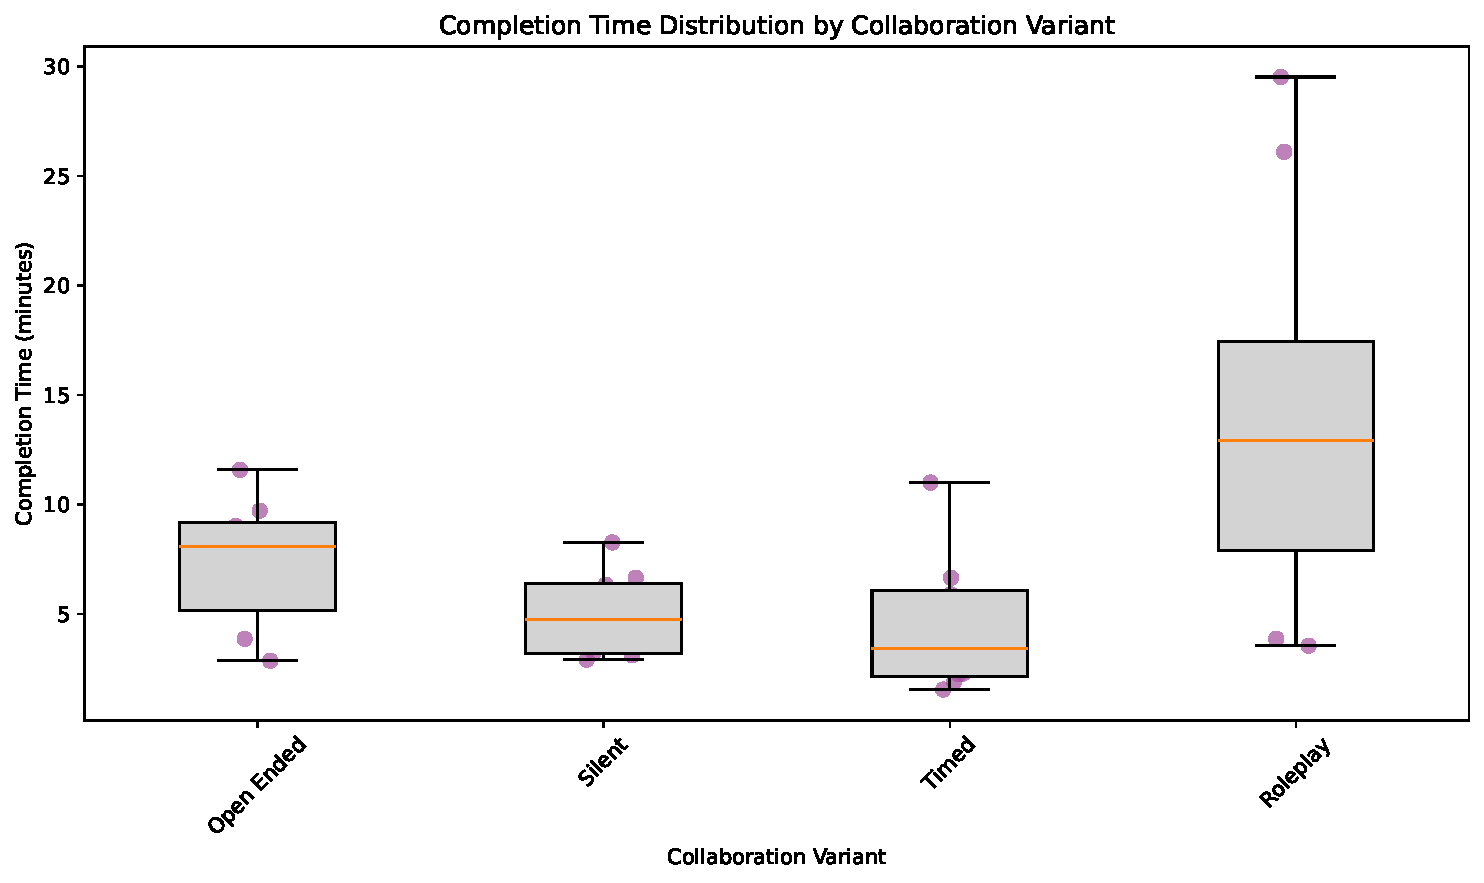
\includegraphics[width=0.7\textwidth]{assets/06/completion_time_by_variant.pdf}
\caption{Completion times by task variant}
\label{fig:completion_times_main}
\end{figure}

\begin{table}[h]
\centering
\caption{Completion Time Statistics by task variant}
\label{tab:completion_time_stats}
\begin{tabular}{lrrrr}
\toprule
\textbf{Variant} & \textbf{Mean (min)} & \textbf{SD} & \textbf{Median} & \textbf{Range} \\
\midrule
Silent & 5.00 & 1.95 & 4.76 & 2.92-8.27 \\
Timed & 4.52 & 3.26 & 3.74 & 1.55-11.00 \\
Open Ended & 7.35 & 2.99 & 7.24 & 2.87-11.58 \\
Roleplay & 14.09 & 9.45 & 12.72 & 3.55-29.52 \\
\bottomrule
\end{tabular}
\end{table}

The Silent condition achieved the most consistent efficiency (lowest variance), while Roleplay showed extreme variability, with completion times ranging from 3.55 to 29.52 minutes. Post-hoc Wilcoxon signed-rank tests identified significant pairwise differences: Roleplay was significantly slower than Silent (W=2, p=0.023, r=0.80, large effect) and Timed (W=0, p=0.008, r=0.94, large effect).

\subsubsection{Silent vs. Verbal Communication Comparison}

Examining the relationship between communication modality and task efficiency reveals a more complex pattern than a simple verbal vs. non-verbal dichotomy. While the Silent condition (5.00 minutes) outperformed unconstrained verbal communication (Open Ended: 7.35 minutes), the fastest completion times occurred under the Timed condition (4.52 minutes), which maintained verbal communication but imposed external time pressure.

Comparing Silent to the two unconstrained verbal conditions (Open Ended and Roleplay) yields a combined mean of 10.72 minutes (Mann-Whitney U = 27.0, p = 0.025, r = 0.46, medium effect), supporting the hypothesis that unconstrained verbal communication can introduce coordination overhead.

\subsubsection{Time Pressure Effects}
The Timed condition demonstrated that external time pressure can drive efficiency without significantly compromising task success (6/8 completions). Despite the fastest mean completion time (4.52 minutes), the high variance (SD = 3.26) indicates that time pressure affected dyads differently.

\subsubsection{Role Conflict Impact}

The Roleplay condition, which introduced artificial role conflicts, showed the poorest performance overall. The high variance suggests that some dyads adapted better to conflicting objectives than others, with completion times varying by nearly an order of magnitude.

\subsubsection{Environmental Consistency}\label{sec:environments}

Virtual environments showed no significant performance differences, confirming equivalent difficulty levels as intended (detailed analysis in Section~\ref{sec:env-order-effects}).

\subsubsection{Learning and Order Effects}\label{sec:learning}

Latin square randomization successfully controlled for systematic order effects, though variant-specific learning patterns emerged (detailed analysis in Section~\ref{sec:env-order-effects}).

\section{Bridge Quality Analysis}\label{sec:bridge_quality}

\begin{table}[!t]
\centering
\caption{Bridge Quality and Construction Patterns}
\label{tab:bridge_construction_summary}
\begin{tabular}{@{}p{3.2cm}p{5.5cm}p{3.2cm}p{2.3cm}@{}}
\toprule
\textbf{Finding} & \textbf{Description} & \textbf{Result} & \textbf{Section} \\
\midrule
\textbf{Quality-Speed Independence} & No significant correlation between completion time and structural performance (medium effect sizes suggest insufficient power) & All FEA metrics p > 0.25, W = 0.13-0.23 & \ref{sec:bridge_quality} \\
\textbf{Construction Efficiency Under Pressure} & Time constraints improved mean resource usage efficiency & 81\% vs 48\% mean usage rate & \ref{appendix:construction} \\
Block Type Strategy & Timed condition favored simple plank elements for efficiency & 48.6\% planks (Timed variant) & \ref{appendix:construction} \\
Ground-Level Design Preference & Most bridges built at minimal height for cost efficiency & Mean height 30.33 cm & \ref{appendix:construction} \\
\textbf{Resource Waste by Constraint} & Roleplay generated most object spawning relative to usage & 26.2 vs 11.6 spawned/used ratio & \ref{appendix:construction} \\
\bottomrule
\end{tabular}
\end{table}

\subsection{Structural Performance Results}

Bridge quality analysis covered 30/32 successfully completed structures using finite element analysis with three metrics: Safety Factor (structural capacity), von Mises stress (stress distribution), and displacement (stiffness).

\subsubsection{Independence of Quality and Speed}

Despite 3× differences in completion times, structural quality showed no statistically significant variant effects. Safety Factor showed no significant differences across variants ($\chi^2$ = 4.062, p = 0.255, Kendall's W = 0.226, medium effect), though the medium effect size suggests potential differences that this study lacked adequate power (34\% for medium effects) to reliably detect. Similarly, von Mises stress distributions remained statistically equivalent ($\chi^2$ = 3.200, p = 0.362, Kendall's W = 0.178, medium effect), and displacement measurements showed no significant variation ($\chi^2$ = 2.288, p = 0.515, Kendall's W = 0.127, medium effect). Construction cost analysis also revealed no significant differences between variants ($\chi^2$ = 3.120, p = 0.373, Kendall's W = 0.173, medium effect).

\subsubsection{Construction Patterns}

Resource utilization patterns differed systematically across task variants. The Timed condition achieved the highest efficiency with 81\% object usage, as participants favored simple structural elements to meet time demands. The Open Ended condition showed the lowest efficiency at 48\% usage, reflecting more exploratory construction approaches. Silent and Roleplay conditions exhibited intermediate utilization patterns between these extremes.

Complete bridge quality data and additional structural analysis details are provided in Appendix~\ref{appendix:bridge_quality_results}.

\section{Collaboration Dynamics}

\subsection{Movement Patterns and Activity Levels}\label{sec:movement}

\begin{table}[!t]
\centering
\caption{Movement Patterns and Activity Levels}
\label{tab:movement_summary}
\begin{tabular}{@{}p{3.2cm}p{5.5cm}p{3.2cm}p{2.3cm}@{}}
\toprule
\textbf{Finding} & \textbf{Description} & \textbf{Result} & \textbf{Section} \\
\midrule
\textbf{Partner Activity Correlation} & Strong correlation between partners' total movement distances & $\rho$ = 0.737 (p < 0.001) & \ref{sec:movement} \\
Speed Consistency & Average movement speed remained stable across variants & Friedman $\chi^2$ = 3.750, p = 0.290 & \ref{sec:movement} \\
\textbf{Activity Level Asymmetry} & Roleplay condition showed most unbalanced movement patterns & Mean asymmetry 0.71 vs 0.32 & \ref{sec:movement} \\
Dyad Activity Patterns & Individual partnerships maintained consistent activity level patterns & $\rho$ = 0.737 across variants & \ref{appendix:movement_communication} \\
Individual Movement Variability & Wide differences in total spatial activity between participants & 33.87-515.28 meters range & \ref{appendix:movement_communication} \\
Speed-Performance Trend & Marginal negative correlation between speed and completion time & $\rho$ = -0.332 (p = 0.064) & \ref{appendix:movement_communication} \\
\bottomrule
\end{tabular}
\end{table}

\subsubsection{Partner Activity Level Correlation}

Analysis of partner movement patterns revealed that the correlation between partners' total movement distances—measuring whether both participants exhibited similar activity levels during sessions—showed strong overall correlation ($\rho$ = 0.737, p < 0.001, r² = 0.543, large effect). This metric captures whether one partner's high or low activity levels were matched by their partner's activity levels.

The strength of this activity level correlation varied across collaboration variants, ranging from near-perfect matching under time pressure ($\rho$ = 0.939, r² = 0.881) to much weaker matching in silent conditions ($\rho$ = 0.351, r² = 0.123). Since correlations are calculated between partners within the same session (who share identical session durations), these differences reflect genuine coordination patterns rather than duration effects. This suggests that different task variants influence whether partners engage with similar intensity levels (see Table \ref{tab:movement_sync}).

\begin{table}[htbp]
\centering
\caption{Movement Activity Level Correlation by task variant}
\label{tab:movement_sync}
\begin{tabular}{lrrrl}
\toprule
\textbf{Variant} & \textbf{Correlation} & \textbf{p-value} & \textbf{r²} & \textbf{Interpretation} \\
\midrule
Timed & 0.939 & 0.001 & 0.881 & Near-perfect activity matching \\
Open Ended & 0.890 & 0.003 & 0.792 & Strong activity level matching \\
Roleplay & 0.658 & 0.076 & 0.434 & Moderate activity matching \\
Silent & 0.351 & 0.394 & 0.123 & Weaker activity matching \\
\bottomrule
\end{tabular}
\end{table}

Individual dyads showed consistent activity level patterns across variants, suggesting stable partnership activity characteristics.

\subsubsection{Movement Speed Analysis}

Average movement speed remained consistent across variants (Friedman $\chi^2$ = 3.750, p = 0.290), confirming that coordination rather than activity level drives performance differences.

Detailed movement analysis and session-by-session data are provided in Appendix~\ref{appendix:movement_results}.

\subsection{Communication Patterns}\label{sec:communication}

\begin{table}[!t]
\centering
\caption{Communication and Collaboration Dynamics}
\label{tab:communication_summary}
\begin{tabular}{@{}p{3.2cm}p{5.5cm}p{3.2cm}p{2.3cm}@{}}
\toprule
\textbf{Finding} & \textbf{Description} & \textbf{Result} & \textbf{Section} \\
\midrule
\textbf{Speaking Rate Stability} & Words per minute remained consistent regardless of variant & 70.85 mean WPM (p = 0.687) & \ref{sec:communication} \\
\textbf{Spatial Reference Stability} & Percentage of spatial references remained constant across variants & 6.5\% mean (p = 0.882) & \ref{sec:communication} \\
\textbf{Strategic Planning Consistency} & Planning vs execution communication ratio remained stable across variants & 32\% planning, 68\% execution (p = 0.687) & \ref{sec:communication} \\
\bottomrule
\end{tabular}
\end{table}

Communication analysis covered 24 sessions with verbal interaction (Silent condition excluded by design).

\subsubsection{Spatial Language Patterns}

Analysis of spatial coordination language revealed consistent patterns across verbal communication variants. Spatial references (words like "here," "there," "this," "that," and directional terms) comprised approximately 6.5\% of all verbal communication, with this proportion remaining stable across Open Ended, Timed, and Roleplay conditions despite differences in session duration and total word counts.

This consistency suggests that spatial coordination language represents a fundamental communication requirement, independent of task variants or total verbal activity levels.

\subsubsection{Strategic Planning Patterns}
Communication pattern analysis examined the distribution between planning-related and execution-related language across verbal variants. When categorizing utterances containing planning markers (words like "plan," "strategy," "should," "let's," "how about," "what if," "we could") versus execution markers (words like "put," "place," "move," "grab," "take," "drop"), the ratio remained consistent across Open Ended, Timed, and Roleplay conditions at approximately 32\% planning-focused communication versus 68\% execution-focused communication.

Complete transcript analysis and communication statistics are provided in Appendix~\ref{appendix:communication_results}. The specific word lists and coding categories used for this analysis are documented in Appendix~\ref{appendix:coding_categories}.


\section{System Performance Validation}\label{sec:system_performance}

\begin{table}[!t]
\centering
\caption{System Performance and User Experience}
\label{tab:system_experience_summary}
\begin{tabular}{@{}p{3.2cm}p{5.5cm}p{3.2cm}p{2.3cm}@{}}
\toprule
\textbf{Finding} & \textbf{Description} & \textbf{Result} & \textbf{Section} \\
\midrule
Spatial Tracking Reliability & No reported tracking drift across all study sessions & Zero critical failures, only minor drift & \ref{sec:system_performance} \\
Network Performance & Latency remained below human perception thresholds & Zero problematic disruptions & \ref{sec:system_performance} \\
\textbf{System Usability Learning Effect} & Significant improvement in interface usability over sessions & 67.5 → 72.5 mean SUS & \ref{sec:usability} \\
\textbf{Experience Level Benefits} & Limited AR/VR users showed strongest usability improvements & +9.6 vs +5.0 point gains & \ref{appendix:subjective} \\
Cognitive Workload Stability & Mental effort requirements remained consistent across sessions & NASA-TLX p = 0.597 & \ref{appendix:subjective} \\
Relationship Dynamics Stability & Partnership quality remained stable throughout study & 3.69 → 3.75 mean IOS & \ref{appendix:subjective} \\
\bottomrule
\end{tabular}
\end{table}

\subsection{Technical Architecture Performance}

System performance met design requirements with some areas for refinement:
\begin{itemize}
\item \textbf{Spatial tracking}: Performance was reliable overall, with minor drift occurring in 2 sessions and users generally disliking the frequent calibration procedures
\item \textbf{Network synchronization}: Latency remained mostly below perceptual thresholds, with occasional network fluctuations being perceptible but not disruptive
\item \textbf{Interaction precision}: Grid-snapping enabled effective construction of stable structures, though some participants noted trade-offs in fine-grained placement control
\end{itemize}

\subsection{Usability and Learning}\label{sec:usability}

\subsubsection{System Usability Scale Progression}

SUS scores improved significantly (67.5 → 72.5, t = 2.760, p = 0.015, Cohen's d = 0.98, large effect), with learning effects strongest for users with limited AR/VR experience (+9.6 points) and no experience (+5.0 points), while moderate experience participants exhibited a slight decline in satisfaction (-1.0 points).

\subsubsection{Cognitive Workload Stability}

NASA-TLX scores remained stable across sessions (no significant change from first to last), indicating consistent cognitive demands despite improving proficiency.

\section{Individual Differences and Adaptation}\label{sec:individual_differences}

\begin{table}[!t]
\centering
\caption{Individual Differences and Qualitative Insights}
\label{tab:individual_qualitative_summary}
\begin{tabular}{@{}p{3.2cm}p{5.5cm}p{3.2cm}p{2.3cm}@{}}
\toprule
\textbf{Finding} & \textbf{Description} & \textbf{Result} & \textbf{Section} \\
\midrule
\textbf{Limited Power for Personality Effects} & Big Five traits showed weak-moderate correlations but insufficient power to detect significance & All |$\rho$| < 0.41, p > 0.10 (51\% power for $\rho$=0.5) & \ref{sec:individual_differences} \\
Openness as Strongest Predictor & Most substantial personality-performance relationship (still weak) & $\rho$ = -0.409 (p = 0.115) & \ref{appendix:individual_differences} \\
Age-Performance Trend & Moderate positive correlation between age and completion time & $\rho$ = 0.424 (p = 0.101) & \ref{appendix:individual_differences} \\
Gender Performance Similarity & Male and female participants performed similarly & 7.89 vs 7.59 mean minutes & \ref{appendix:participants} \\
\bottomrule
\end{tabular}
\end{table}

\subsection{Personality Effects}

Analysis of Big Five personality traits revealed weak correlations with both task completion time and bridge structural quality:

\textbf{Task Completion Time correlations:}
\begin{itemize}
\item Extraversion: $\rho$ = -0.111 (p = 0.682)
\item Openness: $\rho$ = -0.409 (p = 0.115)
\item Conscientiousness: $\rho$ = -0.009 (p = 0.974)
\item Agreeableness: $\rho$ = -0.036 (p = 0.895)
\item Neuroticism: $\rho$ = -0.116 (p = 0.668)
\end{itemize}

\textbf{Bridge Quality correlations:}
\begin{itemize}
\item Extraversion: $\rho$ = -0.034 (p > 0.10)
\item Openness: $\rho$ = 0.122 (p > 0.10)
\item Conscientiousness: $\rho$ = 0.089 (p > 0.10)
\item Agreeableness: $\rho$ = 0.201 (p > 0.10)
\item Neuroticism: $\rho$ = -0.156 (p > 0.10)
\end{itemize}

While none reached statistical significance, distinct patterns emerged that warrant cautious interpretation given the study's limited statistical power. For task speed, Openness showed the strongest relationship ($\rho$ = -0.409, r² = 0.167, medium effect), suggesting that individuals more open to new experiences may adapt more quickly to the collaborative AR construction task. For structural quality, Agreeableness showed the strongest relationship ($\rho$ = 0.201, r² = 0.040, small effect), suggesting that more agreeable individuals may contribute to better collaborative construction outcomes.

\subsection{Experience Level Effects}

AR/VR experience showed complex non-linear relationships with both task performance and learning outcomes. The sample comprised 3 participants with no experience, 11 with limited experience, and 2 with extensive experience.

\textbf{Task Completion Performance by Experience Level:}
\begin{itemize}
\item No Experience: Mean completion time = 7.28 $\pm$ 3.12 minutes
\item Limited Experience: Mean completion time = 7.85 $\pm$ 2.89 minutes  
\item Moderate Experience: No participants in this category
\item Extensive Experience: Mean completion time = 6.41 $\pm$ 2.15 minutes
\end{itemize}

As expected, the data revealed that participants with extensive experience achieved the fastest completion times.

\subsection{Multivariate Predictive Models}
To examine whether combinations of individual difference variables could better predict collaboration outcomes than single factors, three linear regression models were constructed using personality traits, demographics, and experience as predictors.

\subsubsection{Model Specifications}

\textbf{Model 1: Task Performance Prediction}
\begin{align}
\text{Completion Time} = \beta_0 &+ \beta_1 \text{Agreeableness} + \beta_2 \text{Conscientiousness} \nonumber \\
&+ \beta_3 \text{Extraversion} + \beta_4 \text{Neuroticism} + \beta_5 \text{Openness} \nonumber \\
&+ \beta_6 \text{Age} + \beta_7 \text{Gender} + \beta_8 \text{AR Experience} + \epsilon
\end{align}

\textbf{Model 2: Learning Prediction}
\begin{align}
\text{SUS Progression} = \beta_0 &+ \beta_1 \text{Initial SUS} + \beta_2 \text{AR Experience} \nonumber \\
&+ \beta_3 \text{Agreeableness} + \beta_4 \text{Conscientiousness} \nonumber \\
&+ \beta_5 \text{Extraversion} + \beta_6 \text{Neuroticism} + \beta_7 \text{Openness} + \epsilon
\end{align}

\textbf{Model 3: Bridge Quality Prediction}
\begin{align}
\text{Safety Factor} = \beta_0 &+ \beta_1 \text{Completion Time} + \beta_2 \text{AR Experience} \nonumber \\
&+ \beta_3 \text{Agreeableness} + \beta_4 \text{Conscientiousness} \nonumber \\
&+ \beta_5 \text{Extraversion} + \beta_6 \text{Neuroticism} + \beta_7 \text{Openness} + \epsilon
\end{align}

\subsubsection{Model Performance}

All three models demonstrated poor predictive performance and failed to achieve statistical significance, reflecting the fundamental challenge of multivariate modelling with small sample sizes.

\begin{table}[h]
\centering
\caption{Multivariate Regression Model Summary}
\label{tab:multivariate_regression_summary}
\begin{tabular}{lrrrrl}
\toprule
\textbf{Model} & \textbf{n} & \textbf{R²} & \textbf{Adj. R²} & \textbf{F} & \textbf{p-value} \\
\midrule
Task Performance & 16 & 0.417 & -0.250 & 0.625 & 0.739 \\
Learning (SUS Progression) & 16 & 0.345 & -0.228 & 0.602 & 0.741 \\
Bridge Quality & 16 & 0.350 & -0.218 & 0.616 & 0.731 \\
\bottomrule
\end{tabular}
\end{table}

The negative adjusted R² values indicate severe overfitting, where the number of predictors (7-8 variables) approaches the sample size (n=16), violating the general guideline of 10-15 observations per predictor for stable regression estimates.

\subsubsection{Coefficient Patterns}

Despite poor overall model fit, examination of individual coefficients reveals consistent patterns that align with univariate findings:

\textbf{Task Performance Model:} Openness emerged as the strongest predictor ($\beta$ = -3.161), consistent with the univariate correlation finding ($\rho$ = -0.409).

\textbf{Learning Model:} Neuroticism showed the strongest negative effect ($\beta$ = -5.699) on SUS progression.

\textbf{Bridge Quality Model:} Neuroticism again exhibited strong negative effects ($\beta$ = -3.878), while completion time showed minimal influence ($\beta$ = -0.225).

\subsubsection{Limitations}

These findings underscore the power limitations identified in Appendix~\ref{appendix:power_analysis}, where adequate power for detecting medium personality effects would require samples of 50+ participants. The multivariate models should therefore be interpreted as exploratory analyses that identify potential relationships for future investigation rather than definitive predictive tools.

\begin{figure}[htbp]
\centering
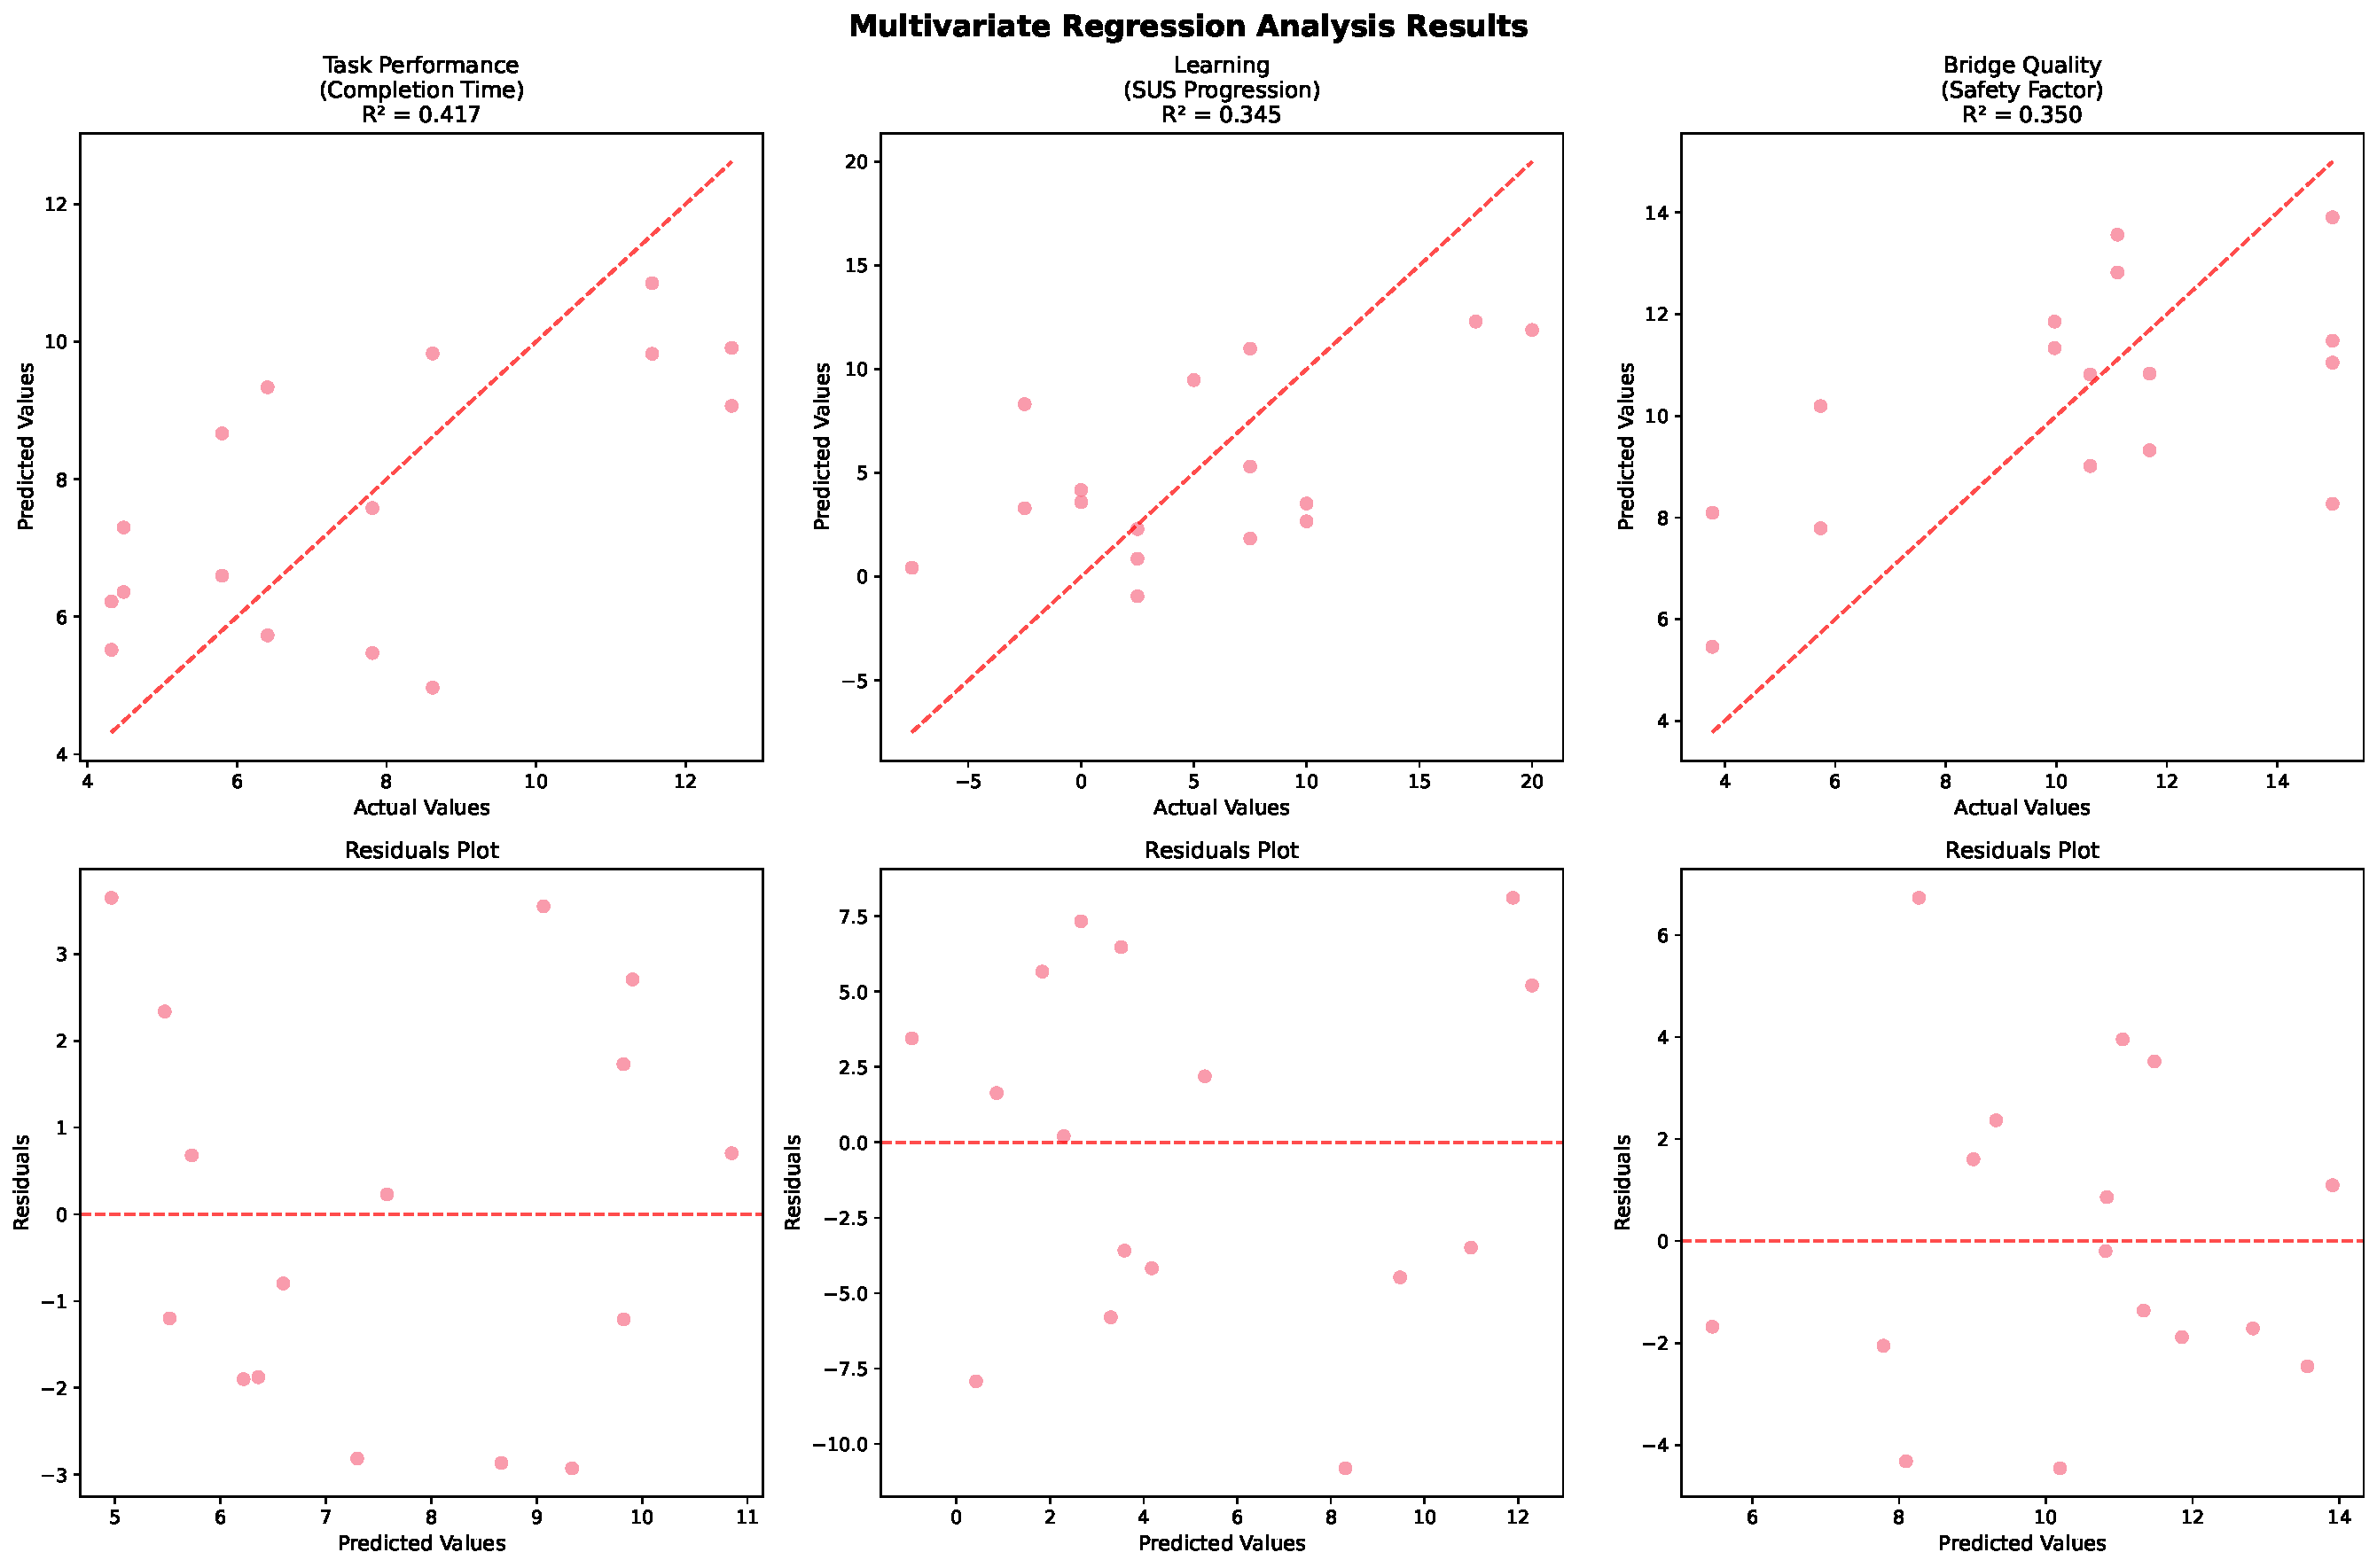
\includegraphics[width=0.9\textwidth]{assets/06/multivariate_regression_analysis.pdf}
\caption{Multivariate regression analysis results showing predicted vs. actual values (top row) and residual plots (bottom row) for task performance, learning progression, and bridge quality models. Poor model fit is evident from scattered data points around the perfect prediction line and non-random residual patterns, confirming the inadequacy of multivariate approaches with the current sample size.}
\label{fig:multivariate_regression_analysis}
\end{figure}

\subsection{Demographic Patterns}

Age showed moderate correlation with completion time ($\rho$ = 0.424, p = 0.101). Gender differences were minimal. Most participants were German-speaking STEM students (81\%), potentially limiting generalizability.

\section{Environmental and Order Effects}\label{sec:env-order-effects}

\subsection{Virtual Environment Analysis (\textit{Confirmatory})}

Virtual environments showed no significant performance differences (Friedman $\chi^2$ = 2.250, df = 3, p = 0.522, Kendall's W = 0.094, small effect), confirming that the four virtual environments achieved equivalent difficulty levels as intended in the study design. This validates the experimental design goal of creating environments with comparable task demands while providing visual variety to maintain participant engagement.

\subsection{Task Order and Latin Square Effects}

Overall task position effects were non-significant ($\chi^2$ = 2.700, df = 3, p = 0.440, Kendall's W = 0.113, small effect), indicating that the Latin square randomization successfully controlled for learning effects at the aggregate level. However, examination of position-time correlations within each variant revealed different learning patterns.

\begin{table}[h]
\centering
\caption{Learning Effects by Task Variant}
\label{tab:learning_effects}
\begin{tabular}{lrrl}
\toprule
\textbf{Variant} & \textbf{Correlation (r)} & \textbf{p-value} & \textbf{Pattern} \\
\midrule
Open Ended & -0.623 & 0.099 & Strong improvement trend \\
Timed & -0.650 & 0.081 & Strong improvement trend \\
Silent & -0.023 & 0.959 & No learning effect \\
Roleplay & 0.016 & 0.971 & No learning effect \\
\bottomrule
\end{tabular}
\end{table}

The verbal conditions (Open Ended, Timed) showed stronger learning effects than the constrained conditions (Silent, Roleplay), suggesting that practice benefits may be more pronounced when participants can freely communicate and adapt their strategies. The Latin square design prevented systematic position bias while allowing detection of these variant-specific learning patterns.

\section{Qualitative Themes and Adaptation Patterns}\label{sec:qualitative}

Post-study interviews with all 16 participants and 8 dyads revealed distinct behavioral themes and adaptation strategies that emerged across the collaborative AR experience. Rather than focusing on individual responses, this analysis identifies patterns that appeared consistently across multiple participants and sessions.

\subsection{The Bridge Definition}

The most significant and unexpected theme involved fundamental disagreements about what exactly constitutes a "bridge".

\textbf{Engineering Traditionalists} maintained that bridges must incorporate vertical structural elements and clear elevation above the ground plane. As one participant argued: \textit{"For me a bridge has a pole and it has to lift up in the air. Otherwise it would be a road if you just place blocks next to each other"} (Participant 2). This perspective emphasised structural integrity and adherence to real-world engineering principles.

\textbf{Pragmatic Optimisers} discovered that ground-level solutions satisfied task requirements while minimising resource costs. These participants treated the floor as a structural foundation: \textit{"We aligned on the idea, that we can just exploit the system in a way that we should build around and use the floor as a stability measure"} (Participant 5).

Most dyads evolved from initial engineering idealism toward pragmatic compromise, demonstrating how collaborative pressure and performance metrics can override individual technical preferences. This persisted across all task variants.

\subsection{Template Development and Cross-Variant Learning}

Participants developed reusable construction templates across task variants. Six of eight dyads completed the Silent condition within the time limit.

\textbf{Template Development Observed}: Dyads established base designs through iterative refinement: \textit{"Once you figured out a good base design you can iterate from that and that worked very well with the partner"} (Participant 1).

\textbf{Cross-Variant Learning}: Participants referenced prior experience in later variants: \textit{"In the silent task because in the first task we kind of agreed on how a bridge should look like... so in the second task we could just easily build the bridge and everyone knew what was to do"} (Participant 1).

\subsection{Communication Patterns Under Different Constraints}

Different collaboration constraints produced distinct communication adaptations.

\textbf{Time Pressure Effects}: \textit{"We were very efficient uh we we had no extra conversations you know it was exactly on point we agreed very fast"} (Participant 4).

\textbf{Silent Collaboration}: Multiple dyads reported successful execution without verbal communication, with participants referencing spatial positioning and gestural coordination.

\textbf{Role Conflict Effects}: The Roleplay variant created reported coordination difficulties: \textit{"It was harder... especially like if you have small pieces to align them correctly... in the end I was more a bit frustrated because it was like hard especially like if you have different interests as well"} (Participant 1).

\subsection{Technical Adaptation Patterns}

Participants showed varying responses to technical limitations throughout the study.

\textbf{Learning Effects Reported}: Initial difficulty with block placement decreased over time: \textit{"At the beginning it was more complicated, but at the end 100\%"} (Participant 4).

\textbf{Experience Level Differences}: Participants with AR/VR background reported different expectations: \textit{"I knew that things not always work perfectly 100\% of the time. So I was quite relaxed when stuff didn't work out"} (Participant 1).

\textbf{Role Distribution Observed}: Dyads adapted to individual technical proficiency differences: \textit{"For the person for who the system works best, like took the lead in building and like the other just checked what they were doing"} (Participant 1).

\subsection{Individual Differences in Collaboration}

Participants reported different approaches to collaboration based on personal characteristics.

\textbf{Planning Orientation}: \textit{"The most important trait actually... is being conscientious so um to like plan it well"} (Participant 14).

\textbf{Flexibility Responses}: \textit{"I think I'm a very open person you know when somebody expresses an opinion to me and their opinion is better I can accept that and I go with it"} (Participant 14).

\textbf{Prior Familiarity Effects}: \textit{"Since I know her very good, we're working together, we're colleagues... it was very easy to communicate"} (Participant 8).

\subsection{Observed Collaboration Styles}

Three distinct collaboration patterns emerged across dyads:

\textbf{Pragmatists} prioritised efficiency and resource optimisation, consistently choosing ground-level solutions that satisfied task requirements while minimising costs: \textit{"We aligned on the idea, that we can just exploit the system in a way that we should build around and use the floor as a stability measure"} (Participant 5).

\textbf{Engineers} maintained focus on structural integrity and traditional engineering principles, insisting that bridges incorporate vertical elements: \textit{"For me a bridge has a pole and it has to lift up in the air. Otherwise it would be a road if you just place blocks next to each other"} (Participant 2).

\textbf{Negotiators} emphasised process management and consensus building, spending significant time coordinating approaches before construction and facilitating compromise between different technical preferences.


